\documentclass[12pt]{article}
\usepackage{graphicx, amsmath}
\usepackage{caption}
\usepackage{algorithm}
\usepackage{algpseudocode}
\graphicspath{ {./} }
\setlength{\oddsidemargin}{0.25 in}
\setlength{\evensidemargin}{-0.25 in}
\setlength{\topmargin}{-0.6 in}
\setlength{\textwidth}{6.5 in}
\setlength{\textheight}{8.5 in}
\setlength{\headsep}{0.75 in}
\setlength{\parindent}{0 in}
\setlength{\parskip}{0.1 in}

\begin{document}
\thispagestyle{plain}
   \newpage
   \setcounter{page}{1}
   \noindent
   \begin{center}
   \framebox{
      \vbox{\vspace{2mm}
    \hbox to 6.28in { {\bf BioE 131: Intro to Computational Biology}
                        \hfill Fall 2020 }
       \vspace{4mm}
       \hbox to 6.28in { {\bf \Large \hfill Grammars and Automata  \hfill} }
       \vspace{2mm}
       \hbox to 6.28in { {\it Professor: Ian Holmes \hfill} }
      \vspace{2mm}}
   }
   \end{center}
   {Notes written by Vikram Shivakumar}
   \vspace*{4mm}


\section{Introduction}
In previous notes, we encountered models like finite state machines and HMMs, which provide a set of states that can be traversed. These models fall uder a broader category of abstract machines called \textbf{automata}. These models are also closely related to the concept of \textbf{grammars}, which are used in computer science and linguistics to describe syntactic structure. In this note, we will discuss grammars and automata, and how they are related to the many algorithms and models we've previously discussed.
\section{Grammars}
A grammar is a system or set of rules to generate a string of a particular pattern. One type we are all familiar with is the grammar of a language, which dictates the certain patterns that are allowed (adjective before noun, direct object after transitive verb, etc). But this idea can extend to other areas, for example music, graphics, and of course bioinformatics.
\subsection{Terminology}
First some terms to be familiar with: \textbf{terminal symbols} and \textbf{nonterminal symbols} represent the elements of the grammar rules, called \textbf{production rules}. Each production rule is of the form $LHS \longrightarrow RHS$, representing a transformation from the left-hand side of the rule (LHS) to the right hand side (RHS). These rules can be repeatedly applied on nonterminal symbols, until only terminal symbols remain. For example, the following is a grammar for RNA structure:
$$\text{Non-terminal symbols } = \{S\}$$
$$\text{Terminal symbols } = \{A, C, G, U, \epsilon\}$$
$$\text{Rules: } \begin{array}{@{}c@{}}
    S \rightarrow SA \text{ or } AS\\
    S \rightarrow SC \text{ or } CS \\
    S \rightarrow SG \text{ or } GS \\
    S \rightarrow SU \text{ or } US \\
    S \rightarrow ASU \\
    S \rightarrow USA \\
    S \rightarrow GSC \\
    S \rightarrow CSG \\
    S \rightarrow SS \\
    S \rightarrow \epsilon
    \end{array}$$
In this grammar, the rules represent unpaired and paired bases, and the terminal symbol $\epsilon$ represents allows for sequence termination. Figure \ref{fig:rna} shows how these rules can be used to generate a structure.
\begin{figure}[ht]
    \centering
    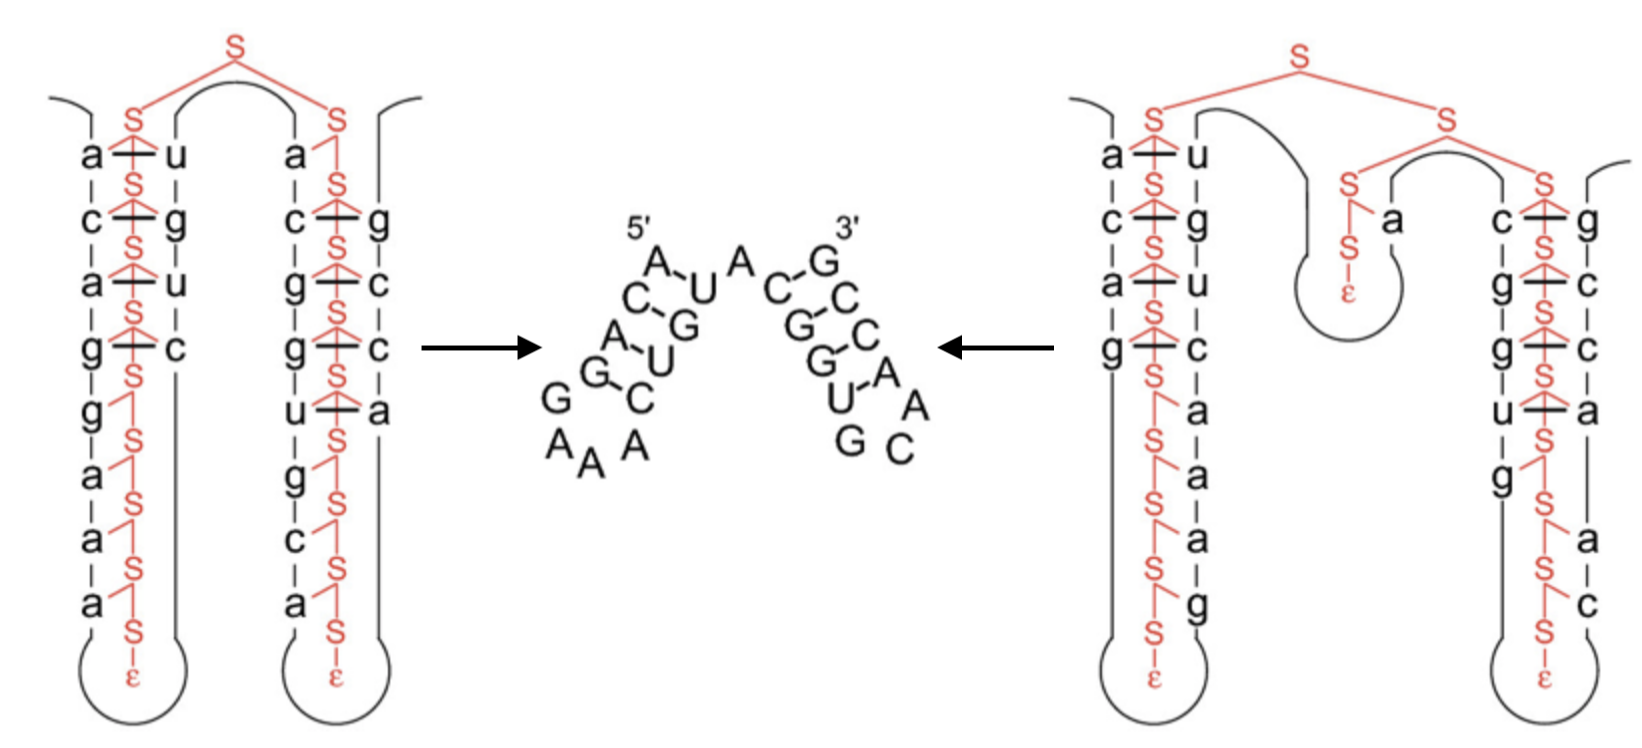
\includegraphics[width=.9\linewidth]{rna.png}
    \caption{Different derivations leading to the same structure}
    \label{fig:rna}
\end{figure}

\subsection{Chomsky hierarchy}
The Chomsky hierarchy is a classification of different types of grammars, which differ in the allowable production rules.
\subsubsection{Regular grammars}
Regular grammars are the lowest level type of grammar in the hierarchy, and thus the most constrained in the types of production rules. In these grammars, two types of rules are allowed:
$$A \rightarrow xB$$
$$A \rightarrow \epsilon$$
where $A$ and $B$ are nonterminals and $x$ is any terminal symbol (and $\epsilon$ is an empty string). These grammars can define strings of various items (terminal symbols), which is useful in many scenarios. One common usage of regular grammars is in \textbf{regular expressions (regex)}, where a query string pattern can be used to search in large strings. For example, if we are searching for a sequence motif of 6 Cs, followed by a variable-length TATA repeat region, followed by the motif ATGG and variable region between 10 and 20nt, lastly ending with a nonzero-length stretch of Ts, we could define the regular expression: ``C\{6\}(TATA)+ATGG.\{10,20\}T+". Notice this expression has a series of \textbf{states} (e.g. TATA repeat, variable region), that are in series.\\[10pt]
How would we search for a pattern from a regular grammar (like a regex string) in a large text (like a genome)? We could first scan for the first state in the pattern, and once we find a match, check if the subsequent states match. This is similar to traversing a \textbf{finite state machine}! In fact, regular grammars are \textit{equivalent} to finite state machines.
\begin{figure}[h]
    \centering
    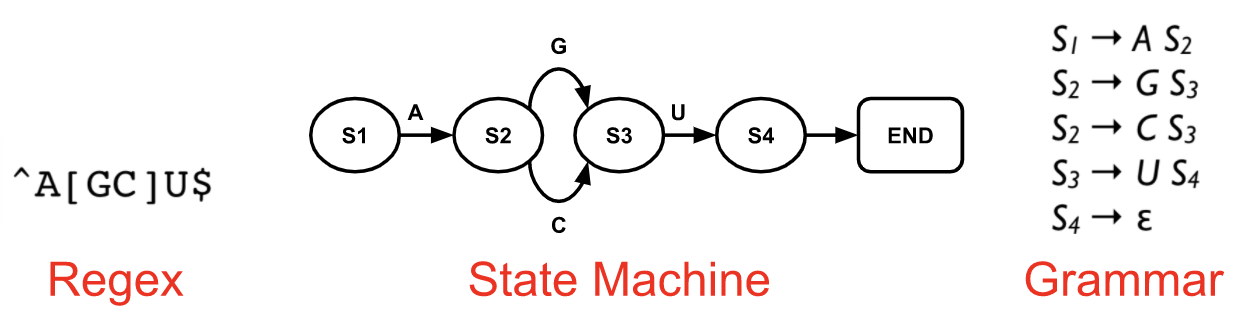
\includegraphics[width=.8\linewidth]{grammar.png}
    \caption{Regular grammars can be represented as FSMs}
    \label{fig:my_label}
\end{figure}\\[10pt]
This is one aspect of a broader connection between grammars and \textbf{automata}, of which a finite state machine is one example. These automata grow more complex with more complex grammars, and often can be used as \textbf{parser algorithms} for a string generated by a corresponding grammar. For example, a finite state machine can be used to parse many types of data which follow a regular grammar (see the note on biological filetypes and pairwise alignment).
\subsubsection{Context-free grammars}
The next level above regular grammars are \textbf{context-free grammars}. These grammars allow any set of symbols (terminal and nonterminal) on the right hand side of production rules, but only nonterminal symbols on the left, e.g. $S \rightarrow ASU$ in the above RNA structure grammar. These grammars can represent \textbf{nested or tree structures}, like RNA foldback structures.\\[10pt]
The corresponding automaton for context-free grammars is a finite state machine with a pushdown stack. Recall that pushdown stacks can be used to parse RNA foldback structures and nested base pairing.

\subsubsection{Context-sensitive and unrestricted grammars}
The last two types of grammars are \textbf{context-sensitive} and \textbf{unrestricted grammars}. Context-sensitive grammars allow nonterminal symbols on either side of a production rules, and can model more complex phenomena like pseudoknot structures in RNA.\\[10pt]
Unrestricted grammars allow any production rules, and can thus model any patterns or structures. This is the highest level of the grammar hierarchy, and thus all grammars are unrestricted grammars. Both unrestricted and context-sensitive grammars are equivalent to \textbf{Turing machines}, which are a type of abstract automata that reads a rolling string of symbols, and manipulates them based on assigned rules.

\subsection{Tree-adjoining grammars}
Tree-adjoining grammars define rules to manipulate parse trees as well, rather than just the string itself. In the grammar hierarchy, they are more complex than context-free grammars, but less complex than context-sensitive grammars.  These grammars can be used to model pseudoknot structures in RNA, or direct repeats (repeat sequences which may have intervening sequences).

\section{Automata}
We've seen how there is a fundamental connection between grammars and automata, where each type of grammar corresponds to an equivalent automaton. Often times, an automaton can be used as a parser for the equivalent grammar. One example which have seen is a finite state machine parsing a regular grammar. 

\begin{table}[h]
\centering
\caption{Grammars and equivalent automata}
\label{tab:automata}
\begin{tabular}{cc}
\textbf{Grammar}  & \textbf{Automata}                      \\ \hline
Unrestricted      & Turing machine                         \\
Context-sensitive & Linear-bounded Turing machine          \\
Context-free      & Finite-state machine w/ pushdown stack \\
Regular           & Finite-state machine                  
\end{tabular}
\end{table}

One detail to note: just as grammars form a hierarchy, so do the corresponding automata.\\[10pt]
Over the course, we have discussed a few different algorithms for problems like sequence alignment, RNA folding prediction, and gene annotation. But these algorithms are also connected to grammars! 
\begin{table}[h]
\centering
\caption{Grammars in bioinformatic algorithms}
\label{tab:connect}
\begin{tabular}{ll}
\multicolumn{1}{c}{\textbf{Algorithm/Model}} & \multicolumn{1}{c}{\textbf{Grammar}} \\ \hline
HMM (profile HMMs, phylogenetic HMMs, etc.)  & Regular                              \\
Needleman-Wunsch, Smith-Waterman, Gotoh      & Regular (pair grammar)               \\
Nussinov, McCaskill, Zuker                   & Context-free                         \\
RNA folding w/ pseudoknots                   & Tree-adjoining                      
\end{tabular}
\end{table}

Table \ref{tab:connect} summarizes how algorithms and models we've covered in previous notes are connected to formal grammars (and thus to automata as well).\\[10pt]
In the case of dynamic alignment algorithms for pairwise alignment, we can model the algorithms with a \textbf{pair grammar}. These grammars (and automata) have two output tapes, which in the case of alignment, records the sequences and gaps. Pair grammars also appear in HMMs, where a \textbf{pair HMM} emits pairs of observable outputs.

\section{Summary}
Grammars and automata are closely related topics that form a framework in which to understand algorithms and models for strings (like biological sequences). Automata like finite state machines and HMMs define an underlying regular grammar which dictates the sequences being modeled. Context-free grammars represent stacked or nested structures like RNA sequences or phylogenetic trees, and thus algorithms like Nussinov or tree-building algorithms follow an underlying context-free grammar structure. Understanding these connections between automata, algorithms, and grammars allows us to develop better models and algorithms in computer science and bioinformatics.
% \section{Automata}
% Let's take a look at a few applications of automata in bioinformatics (most of which we have already seen in previous notes!)
% \subsection{Hidden Markov Models}
% Hidden Markov Models (HMMs), like Markov models, are a type of finite state machine, with states equivalent to nonterminal symbols, and transitions equivalent to production rules. As we've seen, HMMs are useful in many biological contexts, from predicting genes (GENSCAN and Glimmer), to profile HMMs.



\end{document}


%topics not covered:
%connections back to topics like HMMs, FSM, RNA folding DP, alignment like Gotoh/needleman-wunsch
